\documentclass[a4paper,12pt]{article} 

% First, we usually want to set the margins of our document. For this we use the package geometry.
\usepackage[top = 2.5cm, bottom = 2.5cm, left = 2.5cm, right = 2.5cm]{geometry} 
\usepackage[T1]{fontenc}
\usepackage[utf8]{inputenc}

% The following two packages - multirow and booktabs - are needed to create nice looking tables.
\usepackage{multirow} % Multirow is for tables with multiple rows within one cell.
\usepackage{booktabs} % For even nicer tables.

% As we usually want to include some plots (.pdf files) we need a package for that.
\usepackage{graphicx} 

% The default setting of LaTeX is to indent new paragraphs. This is useful for articles. But not really nice for homework problem sets. The following command sets the indent to 0.
% \usepackage{setspace}
% \setlength{\parindent}{0in}
\usepackage{indentfirst}

% Package to place figures where you want them.
\usepackage{float}

% The fancyhdr package let's us create nice headers.
\usepackage{fancyhdr}

\usepackage{xcolor,amsmath,amsthm,algorithm2e,tikz,subcaption}
\RestyleAlgo{ruled}

\definecolor{myRed}{RGB}{211, 31, 17}
\definecolor{myOrange}{RGB}{244, 122, 0}
\definecolor{myLightTeal}{RGB}{98, 200, 211}
\definecolor{myDarkTeal}{RGB}{0, 113, 145}


% To make our document nice we want a header and number the pages in the footer.

\pagestyle{fancy} % With this command we can customize the header style.

\fancyhf{} % This makes sure we do not have other information in our header or footer.

\lhead{\footnotesize Algorithm Design and Analysis(H): Assignment 3}% \lhead puts text in the top left corner. \footnotesize sets our font to a smaller size.

%\rhead works just like \lhead (you can also use \chead)
\rhead{\footnotesize Mengxuan Wu} %<---- Fill in your lastnames.

% Similar commands work for the footer (\lfoot, \cfoot and \rfoot).
% We want to put our page number in the center.
\cfoot{\footnotesize \thepage} 

\begin{document}

\thispagestyle{empty} % This command disables the header on the first page. 

\begin{tabular}{p{15.5cm}}
{\large \bf Algorithm Design and Analysis(H)} \\
Southern University of Science and Technology \\ Mengxuan Wu \\ 12212006 \\
\hline
\\
\end{tabular}

\vspace*{0.3cm} %add some vertical space in between the line and our title.

\begin{center}
	{\Large \bf Assignment 3: Applications of Fast Fourier Transform}
	\vspace{2mm}

	{\bf Mengxuan Wu}
		
\end{center}  

\vspace*{0.4cm}

\section{Convolution}

Convolution is a fundamental arithmetic operation on two functions, which produces a third function.
Suppose we have two discrete functions $f$ and $g$, and we want to calculate the convolution of the two functions.
The convolution of $f$ and $g$ is defined as
\begin{equation*}
	(f * g)(t) = \sum_{\tau = -\infty}^{\infty} f(\tau)g(t - \tau)
\end{equation*}

An easy way to convert a convolution operation to a polynomial multiplication problem is by treating the value of the function as the coefficient of a polynomial.
For example, suppose we have two functions $f = [1, 2, 3]$ and $g = [4, 5, 6]$.
We can convert the two functions to two polynomials $f(x) = 1 + 2x + 3x^2$ and $g(x) = 4 + 5x + 6x^2$.
Then the convolution of $f$ and $g$ is equivalent to the multiplication of the two polynomials $f(x)g(x) = 4 + 13x + 28x^2 + 27x^3 + 18x^4$.
And the coefficients of the result polynomial are the values of the convolution of the two functions, which is $[4, 13, 28, 27, 18]$.

In my opinion, the superiority of the FFT is that it provides a fast way to calculate the convolution of two functions.
Since the convolution operation is essential in multiple fields, combined with the well-known optimization trick of ``making common things fast'', the FFT algorithm has been widely used in many applications.
In most applications listed below, we can find that the FFT algorithm is used to speed up the convolution operation, and further improve the efficiency of the algorithm.

\section{Image Processing and Feature Extraction}

Artificial intelligence and machine learning have been widely used in image processing and feature extraction. 
And one core technique in image processing is using a convolutional neural network (CNN) to extract features from images, which is based on the convolution operation and can be implemented by the Fast Fourier Transform (FFT).

We take the image in Figure \ref{fig:original} as an example.
The image can be represented as a 2D matrix, where each element represents the pixel value of the image.
Suppose we want to blur the image, a natural way is to mix each pixel with its neighbors.
For example, we can let each pixel in the new image be the average of itself and its closest 8 neighbors on each side.

\begin{figure}[H]
	\begin{subfigure}{0.5\textwidth}
		\centering
		
\includegraphics[width=0.8\linewidth]{./original.png}
		\caption{Original Image}
		\label{fig:original}
	\end{subfigure}
	\begin{subfigure}{0.5\textwidth}
		\centering
		
\includegraphics[width=0.8\linewidth]{./box blur.png}
		\caption{Blurred Image}
		\label{fig:box blurred}
	\end{subfigure}
	\caption{Blurring an Image}
\end{figure}

In this case, we define a kernel, which is a $3 \times 3$ matrix with all elements equal to $\frac{1}{9}$.
Then we slide the kernel over the image.
At each position, we multiply the kernel with the image, element-wise, and sum up the results.
The result is the pixel value of the new image at that position.
\begin{equation*}
	a'_{i, j} = \sum_{m = -1}^{1} \sum_{n = -1}^{1} a_{i + m, j + n} \cdot \frac{1}{9}
\end{equation*}

Or more intuitively:
\begin{equation*}
	a'_{i, j} = 
	\begin{bmatrix}
		\frac{1}{9} & \frac{1}{9} & \frac{1}{9} \\
		\frac{1}{9} & \frac{1}{9} & \frac{1}{9} \\
		\frac{1}{9} & \frac{1}{9} & \frac{1}{9} \\
	\end{bmatrix}
	\times_{\text{element-wise}}
	\begin{bmatrix}
		a_{i-1, j-1} & a_{i-1, j} & a_{i-1, j+1} \\
		a_{i, j-1} & a_{i, j} & a_{i, j+1} \\
		a_{i+1, j-1} & a_{i+1, j} & a_{i+1, j+1} \\
	\end{bmatrix}
\end{equation*}

We can do more with the kernel by changing the values of the kernel.
For example, we usually use a kernel with a Gaussian distribution to blur the image, which samples the pixels in a 2D Gaussian distribution.
That means a kernel that takes greater weight in the center and less weight on the edges.

\begin{minipage}{0.5\textwidth}
	\centering
	
\includegraphics[width=0.5\linewidth]{./guassian kernel.png}
	\captionof{figure}{Gaussian Blur Kernel Visualization}
	\label{fig:gaussian blurred}
\end{minipage}
\begin{minipage}{0.5\textwidth}
	\centering
	\resizebox{\textwidth}{!}{
		\begin{tabular}{|c|c|c|c|c|}
			\hline
			0.00296902 & 0.0133062 & 0.0219382 & 0.0133062 & 0.00296902 \\
			\hline 
			0.0133062  & 0.0596343 & 0.0983203 & 0.0596343 & 0.0133062 \\
			\hline 
			0.0219382 &  0.0983203 & 0.162103  & 0.0983203 & 0.0219382 \\
			\hline 
			0.0133062 &  0.0596343 & 0.0983203 & 0.0596343 & 0.0133062 \\
			\hline 
			0.00296902 & 0.0133062 & 0.0219382 & 0.0133062 & 0.00296902 \\
			\hline
		\end{tabular}
	}
	\captionof{table}{Gaussian Blur Kernel Matrix}
\end{minipage}

\vspace{1em}

Now we can talk about feature extraction.
A feature, such as an edge, a corner, or a texture, is a pattern that can be found in an image.
It is common practice to use a CNN to extract features from images.
For example, a \texttt{sobel} kernel, which is a $3 \times 3$ matrix that apply a positive weight to the pixels on one side of the center pixel and a negative weight to the pixels on the other side, can be used to extract edges from an image.

\begin{figure}[H]
	\begin{subfigure}{0.5\textwidth}
		\centering
		
\includegraphics[width=0.5\linewidth]{./sobel 1.png}
		\caption{Horizontal Sobel Kernel (green is positive, red is negative) }
		\label{fig:sobel 1}
	\end{subfigure}
	\begin{subfigure}{0.5\textwidth}
		\centering
		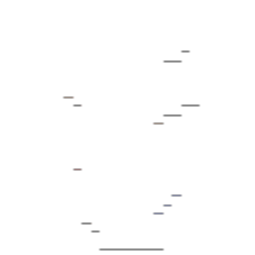
\includegraphics[width=0.5\linewidth]{./sobel 1 e.png}
		\caption{Horizontal edge extracted}
		\label{fig:sobel 2}
	\end{subfigure}
	\caption{Horizontal Edge Extraction}
\end{figure}

\begin{figure}[H]
	\begin{subfigure}{0.5\textwidth}
		\centering
		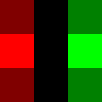
\includegraphics[width=0.5\linewidth]{./sobel 2.png}
		\caption{Vertical Sobel Kernel}
		\label{fig:sobel 3}
	\end{subfigure}
	\begin{subfigure}{0.5\textwidth}
		\centering
		
\includegraphics[width=0.5\linewidth]{./sobel 2 e.png}
		\caption{Vertical edge extracted}
		\label{fig:sobel 4}
	\end{subfigure}
	\caption{Vertical Edge Extraction}
\end{figure}

We can notice that this kernel multiplication is closely related to the convolution operation.
What a kernel do is to multiply the kernel matrix with the image, element-wise, and sum up the results.
If we treat the value of the image as coefficients of a polynomial, and the kernel as another polynomial, then the kernel multiplication is equivalent to the convolution of the two polynomials.
This is where the FFT comes in.

Since CNNs are widely used in image processing, the FFT algorithm can be said to play a crucial role in speeding up the neural network operation.

\section{Signal Processing}

\subsection{Fourier Transform}

The most common application of the FFT is in signal processing, where we use the FFT to analyze the frequency components of a signal.
Given any signal, we can use the FFT to efficiently decompose the signal into multiple frequency components (particularly sine and cosine waves).

Let $f(t)$ be a signal, where $t$ is the time and $f(t)$ is the amplitude of the signal at time $t$.
The Fourier Transform of $f(t)$ is defined as
\begin{equation*}
	F(\omega) = \int_{-\infty}^{\infty} f(t) e^{-i\omega t} dt
\end{equation*}

Since $f(t)$ is always a real number, the final result of the Fourier Transform is a complex number.
The magnitude of the complex number $|F(\omega)|$ represents the amplitude of the frequency component $\omega$ in the signal, or simply to say how strong the frequency component is in the signal.
The phase of the complex number $\angle(F(\omega))$, which corresponds to the angle of the complex number with respect to the real axis, represents the phase shift of the frequency component $\omega$ in the signal.
With the two pieces of information, we can locate each frequency components in the signal.

The Inverse Fourier Transform is defined as
\begin{equation*}
	f(t) = \frac{1}{2\pi} \int_{-\infty}^{\infty} F(\omega) e^{i\omega t} d\omega
\end{equation*}
which is the reverse operation of the Fourier Transform.

\subsection{Discrete Fourier Transform}

In practice, we usually deal with signals that are samples at discrete time points.
The Discrete Fourier Transform (DFT) is a discrete version of the Fourier Transform, which is defined as
\begin{equation*}
	F(k) = \sum_{n=0}^{N-1} f(n) e^{-i2\pi kn/N}
\end{equation*}

We can notice that this formula is very similar to the equation we used to calculate the polynomial multiplication, where we use FFT to convert coefficient representation to point-value representation:
\begin{equation*}
	b_i = \sum_{j=0}^{N-1} a_j e^{-i2\pi j/N}
\end{equation*}
where $a_j$ is the coefficient of the polynomial $a(x)$, and $b_i$ is the point-value representation of the polynomial $b(x)$.
This means that we can use the FFT algorithm to calculate the DFT in $O(N\log N)$ time complexity.

\subsection{Applications}

The applications of the decomposition of signals into frequency components are numerous.
We can take the compression of audio files as an example.
If we see the audio signal as a combination of multiple frequency components, then we don't need to store the entire signal.
Instead, we can store the frequency components with the highest amplitude, and the phase shift of each frequency component.
This is the idea behind the MP3 format, which compresses the audio signal by removing the frequency components with low amplitude.

\section{Image Compression}

One common application of the FFT in image processing is image compression.
A variant of FFT, the Discrete Cosine Transform (DCT), is used in image compression in format like JPEG.
Its core idea is similar to audio compression, where we transform the image matrix into another matrix that represents the frequency components of the image, and then we wipe out the frequency components with lower amplitude.

The formula we use to convert a 2D image matrix $f$ into a 2D frequency matrix $F$ is
\begin{equation*}
	\begin{cases}
		F_{1, 1} = \dfrac1n\sum\limits_{x=1}^n\sum\limits_{y=1}^nf_{x, y} & \\
		F_{1, v} = \dfrac{\sqrt2}n\sum\limits_{x=1}^n\sum\limits_{y=1}^nf_{x, y}\cdot\cos\left(\dfrac{(2y+1)v\pi}{2n}\right) & v = 2, 3, \cdots, n\\
		F_{u, 1} = \dfrac{\sqrt2}n\sum\limits_{x=1}^n\sum\limits_{y=1}^nf_{x, y}\cdot\cos\left(\dfrac{(2x+1)u\pi}{2n}\right) & u = 2, 3, \cdots, n\\
		F_{u, v} = \dfrac2n\sum\limits_{x=1}^n\sum\limits_{y=1}^nf_{x, y}\cdot\cos\left(\dfrac{(2x+1)u\pi}{2n}\right)\cdot\cos\left(\dfrac{(2y+1)v\pi}{2n}\right) & \text{otherwise}
	\end{cases}
\end{equation*}

And the inverse formula is
\begin{align*}
    f_{x, y}&=\dfrac1nF_{1, 1}+\dfrac{\sqrt2}n\sum\limits_{v=2}^nF_{1, v}\cdot\cos\left(\dfrac{(2y+1)v\pi}{2n}\right)+\dfrac{\sqrt2}n\sum\limits_{u=2}^nF_{u, 1}\cdot\cos\left(\dfrac{(2x+1)u\pi}{2n}\right)\\
    &+\dfrac2n\sum\limits_{u=2}^n\sum\limits_{v=2}^nF_{u, v}\cdot\cos\left(\dfrac{(2x+1)u\pi}{2n}\right)\cdot\cos\left(\dfrac{(2y+1)v\pi}{2n}\right)
\end{align*}

A typical DCT matrix after the transformation is shown in Figure \ref{fig:zigzag}.
\begin{figure}[H]
	\centering
	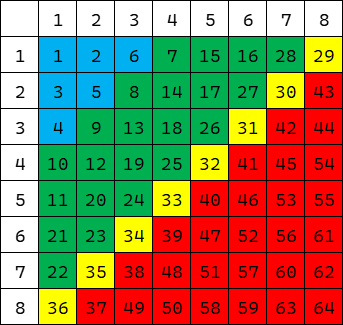
\includegraphics[width=0.5\linewidth]{./DCT.png}
	\caption{Zigzag Order of Frequency Matrix}
	\label{fig:zigzag}	
\end{figure}

To be short, the values in the blue and green areas are the low-frequency components, and the values in the yellow and red areas are the high-frequency components.
Since the human eye is more sensitive to low-frequency components, we can remove the high-frequency components to compress the image (setting the values in the yellow and red areas to zero).
This is part of the idea used in the JPEG compression algorithm.

\section{Probability and Statistics}

FFT is widely used in calculating the frequency distribution of two or more random variables.

For example, suppose we have two random variables $X$ and $Y$.
And we want to calculate the probability distribution of the sum of the two random variables, $Z = X + Y$.
The probability distribution of $Z$ is the convolution of the probability distribution of $X$ and $Y$.
\begin{equation*}
	P(Z = z) = \sum_{x} P(X = x)P(Y = z - x)
\end{equation*}

If the two random variables are discrete, we can treat the probability distribution as a polynomial, and the convolution of the two probability distributions is equivalent to the multiplication of the two polynomials.
Take an example of two independent dice rolls, where $X$ and $Y$ are the random variables representing the results of the two dice rolls.
The probability distribution of $X$ and $Y$ are:
\begin{equation*}
	P(X = x) = 
	\begin{cases}
		\frac16 & x = 1, 2, 3, 4, 5, 6 \\
		0 & \text{otherwise}
	\end{cases}
\end{equation*}

The probability distribution of $Z = X + Y$ is the convolution of the two probability distributions.
We can calculate this by calculating the convolution of the two polynomials.
\begin{equation*}
	\left(\sum_{i = 1}^{6} \frac{1}{6} x^i\right)^2 = \frac{1}{36}x^2 + \frac{1}{18}x^3 + \frac{1}{12}x^4 + \frac{1}{9}x^5 + \frac{5}{36}x^6 + \frac{1}{6}x^7 + \frac{1}{9}x^8 + \frac{5}{36}x^9 + \frac{1}{12}x^{10} + \frac{1}{18}x^{11} + \frac{1}{36}x^{12}
\end{equation*}

The result is the probability distribution of the sum of two dice rolls.
\begin{equation*}
	P(Z = z) = 
	\begin{cases}
		\frac{1}{36} & z = 2 \\
		\frac{1}{18} & z = 3 \\
		\frac{1}{12} & z = 4 \\
		\frac{1}{9} & z = 5 \\
		\frac{5}{36} & z = 6 \\
		\frac{1}{6} & z = 7 \\
		\frac{1}{9} & z = 8 \\
		\frac{5}{36} & z = 9 \\
		\frac{1}{12} & z = 10 \\
		\frac{1}{18} & z = 11 \\
		\frac{1}{36} & z = 12 \\
		0 & \text{otherwise}
	\end{cases}
\end{equation*}

Similar conversion can be done for the difference of two random variables, the product of two random variables, and the ratio of two random variables.
\end{document}